\chapter{Testy i symulacje}
    \section{Czas trwania obliczeń}
        W trakcie projektowania sterowania robota warto uwzględnić wydajność obliczeniową mikrokontrolera. Do obliczenia sterowania wymagana jest duża ilość obliczeń zmiennoprzecinkowych. Obliczenia te pochłaniają większą ilość cykli procesora niż obliczenia całkowitoliczbowe. Aby mieć pewność, że obliczenia zostaną wykonane na czas zdecydowano się porównać różnice wynikające z tego faktu. Wzorzec funkcji testującej został przedstawiony w \ref{list:wzorzecCzasTrwania}.
        
        \begin{lstlisting}[label=list:wzorzecCzasTrwania ,caption=Wzorzec funkcji testującej czas wykonywania obliczeń,  basicstyle=\footnotesize\ttfamily]
        template <typename T>
        u32 calculate(T nr1, T nr2) {
            T temp;
            u32 timerStart = micros();
            for(u32 counter{0}; counter < 1000000; ++counter) {
                temp = nr1 * nr2;
                nr1 += temp;
                nr2 += temp + nr1;
            }
            return micros() - timerStart;
        }
        \end{lstlisting}
        Test przeprowadzono dla wbudowanych typów \verb+int+, \verb+float+ oraz \verb+double+. Każdy test został wykonany 5 razy. Wykonano testy z wyłączoną optymalizacją oraz optymalizacją \texttt{-O3}. Wyniki dla flag \texttt{-O0} przedstawiono w tabeli \ref{tab:czasTrwaniaObliczeńO0}.
        
        \begin{table}[ht]
    		\centering
    		\begin{tabular}{|c|c|c|c|}
                \hline
                \multirow{ 2}{*}{\textbf{Numer testu}} & \multicolumn{3}{c|}{\textbf{Czas trwania obliczeń [\si{\milli\second}]}}     \\ \cline{2-4} 
                & \textbf{int} & \textbf{float}   & \textbf{double}      \\ \hline \hline
                1           & 529,446    & 3482,773 & 4332,720     \\ \hline
                2           & 529,470    & 3482,749 & 4332,743     \\ \hline
                3           & 529,467    & 3482,749 & 4332,743     \\ \hline
                4           & 529,469    & 3482,751 & 4332,743     \\ \hline
                5           & 529,467    & 3482,749 & 4332,744     \\ \hline
                \end{tabular}
    		\caption{Czas trwania obliczeń z wyłączoną optymalizacją (flaga O0)}
    		\label{tab:czasTrwaniaObliczeńO0}
    	\end{table}
        Niestety dla optymalizacji prędkości działania za pomocą flagi \texttt{-O3} nie udało się otrzymać wiarygodnych wyników przedstawioną funkcją. Ze względu na uproszczenia jakich dokonał kompilator, niezależnie od ilości powtórzeń pętli otrzymywany wynik wynosi \SI{0}{\micro\second}. Jednak po dodaniu generatora liczb losowych w postaci modyfikacji kodu z \\ 
        \verb+temp = nr1 * nr2;+ \\ 
        na \\
        \verb+temp = nr1 * nr2 * static_cast<T>(random(100000));+ \\ 
        dla wszystkich testów osiągnięto wyniki rzędu \SI{1180}{\milli\second}. Co pozwala twierdzić, że przy użytej optymalizacji kompilator powinien wystarczająco zoptymalizować kod, tak aby nie wynikały z tego powodu znaczne opóźnienia.
        
        Następne porównanie przeprowadzono po implementacji symulacji sterownika kinematycznego w mikrokontrolerze. Porównano maksymalny czas wykonywania jednej pętli dla flag \texttt{-O0}, \texttt{-Os} i~\texttt{-O3}. Wszystkie zmienne, które zawierają części ułamkowe zostały zdefioniowane jako \texttt{double}. Wyniki przedstawiono w tabeli \ref{tab:czasTrwaniaObliczeńSterownik}.
        \begin{table}[ht]
    		\centering
    		\begin{tabular}{|c|c|c|c|}
                \hline
                \multicolumn{4}{|c|}{\textbf{Czas [\si{\micro\second}]}}     \\ \cline{1-4} 
                 \textbf{-O0} & \textbf{-Os}   & \textbf{-O3} & \textbf{-Ofast}       \\ \hline \hline
                   844    & 452 & 450 & 414     \\ \hline
                \end{tabular}
    		\caption{Czas wykonywania jednej pętli w zależności od optymalizacji}
    		\label{tab:czasTrwaniaObliczeńSterownik}
    	\end{table}
    	
    	Dodatkowo porównano wykorzystanie pamięci przez program. Rozmiar pamięci \texttt{RAM} mikrokontrolera to \SI{20480}{B}, natomiast \texttt{Flash} \SI{65536}{B}.
    	\begin{table}[ht]
    		\centering
    		\begin{tabular}{|c|c|c|c|c|}
                \hline
                \multirow{ 2}{*}{\textbf{Pamięć}} & \multicolumn{4}{c|}{\textbf{Wykorzystanie pamięci}}     \\ \cline{2-5} 
                & \textbf{-O0} & \textbf{-Os}   & \textbf{-O3}   & \textbf{-Ofast}     \\ \hline \hline
                 \textbf{RAM}         & \SI{22.9}{\percent} (\SI{4696}{B})   & \SI{22.9}{\percent} (\SI{4680}{B}) & \SI{22.9}{\percent} (\SI{4680}{B}) & \SI{22.9}{\percent} (\SI{4680}{B})     \\ \hline
                 \textbf{Flash}           & \SI{84.6}{\percent} (\SI{55424}{B})    & \SI{59.0}{\percent} (\SI{38688}{B}) & \SI{62.2}{\percent} (\SI{40736}{B})  & \SI{62.2}{\percent} (\SI{40736}{B})     \\ \hline
                \end{tabular}
    		\caption{Wykorzystanie pamięci w zależności od optymalizacji}
    		\label{tab:wykorzystaniePamieciSterownik}
    	\end{table}
    \section{Symulacja działania sterowania kinematycznego}
        Przed właściwą implementacją sterowania kinematycznego zdecydowano się sprawdzić jego zachowanie za pomocą symulacji komputerowej. Do symulacji wykorzystano oprogramowanie \texttt{Matlab} wraz z pakietem \texttt{Simulink}.
    	Wynik działania dla trajektorii kołowej pokazano na rysunku \ref{fig:trajektoriaKolowaWykres}. Parametry $k1$ i~$k2$ to odpowiednio $0.1$ oraz $1$.
    	\begin{figure}[h]
    		\centering
    		\includegraphics[width=0.45\textwidth]{rys03/trajektoriaKoloWykres.eps}
    		\caption{Porównanie trajektorii pochodzącej z generatora oraz robota}
    		\label{fig:trajektoriaKolowaWykres}
    	\end{figure}
    	
    	Następnie zasymulowano dwa różne sposoby generowania trajektorii poruszania się po pomieszczeniu. Parametry $k1$ i~$k2$ pozostały bez zmian. Wyniki przedstawiono na rysunku \ref{fig:porownanieTrajektorii}.
    	\begin{figure}[h]
			\centering
			\begin{tabular}{@{}ll@{}}
				a) & b) \\
				\includegraphics[width=0.45\textwidth]{rys03/trajektoriaRownoleglek1=02k2=10s1.eps} &
				\includegraphics[width=0.45\textwidth]{rys03/trajektoriaKwadratk1=02k2=10s1.eps} 
			\end{tabular}
			\caption{Porównanie dwóch sposobów generowania trajektorii: a) równoległa b) do środka}
			\label{fig:porownanieTrajektorii}
		\end{figure}
		Wynika z nich, że robot ma tendencję do zaokrąglania gwałtownych zmian ruchu. A w przypadku \ref{fig:porownanieTrajektorii} b) co czwarty zakręt następują załamania rzeczywistego ruchu robota. Po zakończeniu generowania trajektorii robot od razu zatrzymuje się w miejscu bez przeregulowań. 
		
		Następnie zdecydowano się na porównać wpływ parametrów $k1$ i~$k2$ na jakość sterowania. Wyniki dla zmian parametru $k1$, przy stałym $k2 = 1$ pokazano na rysunku \ref{fig:porownanieWplywuParametruk1}.
		\begin{figure}[h]
			\centering
			\begin{tabular}{@{}ll@{}}
				a) & b) \\
				\includegraphics[width=0.45\textwidth]{rys03/trajektoriaRownoleglaPorownaniek1.eps} &
				\includegraphics[width=0.45\textwidth]{rys03/trajektoriaKwadratPorownaniek1.eps}
			\end{tabular}
			\caption{Porównanie wpływu parametru k1 na trajektorię: a) równoległą b) do środka}
			\label{fig:porownanieWplywuParametruk1}
		\end{figure}
		Można z nich wnioskować, że parametr ten ma wpływ na przeregulowania podczas zmian trajektorii. Gdy jest zbyt mały, robot skraca zakręty. Natomiast wraz z~jego wzrostem, robot ma tendencję do coraz większego zaokrąglania zakrętów. Przy dużych wartościach, powstaje także przeregulowanie na prostym odcinku drogi.  
		
		Wyniki dla zmian parametru $k2$, przy stałym $k1=0.1$ zostały przedstawione na rysunku \ref{fig:porownanieWplywuParametruk2}.
		\begin{figure}[h]
			\centering
			\begin{tabular}{@{}ll@{}}
				a) & b) \\
				\includegraphics[width=0.45\textwidth]{rys03/trajektoriaRownoleglaPorownaniek2.eps} &
				\includegraphics[width=0.45\textwidth]{rys03/trajektoriaKwadratPorownaniek2.eps}
			\end{tabular}
			\caption{Porównanie wpływu parametru k2 na trajektorię: a) równoległą b) do środka}
			\label{fig:porownanieWplywuParametruk2}
		\end{figure}
    	Zwiększenie tego parametru powoduje poprawę jakości podążania za zadaną trajektorią. Gdy jest zbyt mały, robot zbyt wcześnie zawraca i następują załamania trajektorii w przypadku trajektorii równoległej. Natomiast w~przypadku trajektorii do środka, następuje zaokrąglenie zakrętów.
    	
    	Znając wpływ parametrów $k1$ i~$k2$ można dobrać ich wartości do robota. Aby było to możliwe należy sprawdzić prędkości obrotowe kół. Powinny być możliwe do zrealizowania przez silniki. Jako parametry testowe wybrano $k1 = 1$ oraz $k2 = 10$. Prędkość postępowa robota wynosi \SI[per-mode=symbol]{1}{\metre\per\second}.
    	\begin{figure}[h]
			\centering
			\begin{tabular}{@{}ll@{}}
				a) & b) \\
				\includegraphics[width=0.45\textwidth]{rys03/trajektoriaRownoleglek1=1k2=10.eps} &
				\includegraphics[width=0.45\textwidth]{rys03/predkosciKolRownoleglek1=1k2=10.eps}
			\end{tabular}
			\caption{Zestawienie: a) Trajektoria równoległa b) Prędkości kół}
			\label{fig:trajektoriaRownoleglaIPredkoscKolk1=1k2=10}
		\end{figure}
		\begin{figure}[h]
			\centering
			\begin{tabular}{@{}ll@{}}
				a) & b) \\
				\includegraphics[width=0.45\textwidth]{rys03/trajektoriaKwadratk1=1k2=10.eps} &
				\includegraphics[width=0.45\textwidth]{rys03/predkosciKolKwadratk1=1k2=10.eps}
			\end{tabular}
			\caption{Zestawienie: a) Trajektoria do środka b) Prędkości kół}
			\label{fig:trajektoriaKwadratIPredkoscKolk1=1k2=10}
		\end{figure}
		Dla obu trajektorii \ref{fig:trajektoriaRownoleglaIPredkoscKolk1=1k2=10} i~\ref{fig:trajektoriaKwadratIPredkoscKolk1=1k2=10} prędkości obrotowe kół dla odcinków prostych wynoszą $\approx~\SI[per-mode=symbol]{4.7}{obr\per\second}$. Natomiast zastosowane silniki według dokumentacji pozwalają na osiągnięcie $\SI[per-mode=symbol]{100}{obr\per\min} = 1\SI[per-mode=symbol, quotient-mode=fraction]{2/3}{obr\per\second}$. Oznacza to, że robot nie jest w stanie poruszać się z taką prędkością. Dodatkowo na zakrętach odnotowywane są skoki prędkości obrotowych. W~przypadku \ref{fig:trajektoriaKwadratIPredkoscKolk1=1k2=10}b) co czwarty zakręt dochodzi do przeregulowań i gwałtownych skoków prędkości obrotowych.
		
		W pierwszej kolejności zdecydowano się zmniejszyć prędkość postępową robota do \SI[per-mode=symbol]{10}{\centi\metre\per\second}. Zmodyfikowano także trajektorię, tak aby odpowiadała szerokości szczotek myjących podłogę.
		\begin{figure}[h]
			\centering
			\begin{tabular}{@{}ll@{}}
				a) & b) \\
				\includegraphics[width=0.45\textwidth]{rys03/trajektoriaRownoleglek1=1k2=10s=01d02.eps} &
				\includegraphics[width=0.45\textwidth]{rys03/predkoscKolRownoleglek1=1k2=10s=01d02.eps}
			\end{tabular}
			\caption{Zestawienie dla prędkości \SI[per-mode=symbol]{10}{\centi\metre\per\second}: a) Trajektoria równoległa b) Prędkości kół}
			\label{fig:trajektoriaRownolegleIPredkoscKolk1=1k2=10s=01d=02}
		\end{figure}
		\begin{figure}[h]
			\centering
			\begin{tabular}{@{}ll@{}}
				a) & b) \\
				\includegraphics[width=0.45\textwidth]{rys03/trajektoriaKwadratk1=1k2=10d02s01.eps} &
				\includegraphics[width=0.45\textwidth]{rys03/predkosciKolKwadratk1=1k2=10d02s01.eps}
			\end{tabular}
			\caption{Zestawienie dla prędkości \SI[per-mode=symbol]{10}{\centi\metre\per\second}: a) Trajektoria do środka b) Prędkości kół}
			\label{fig:trajektoriaKwadratIPredkoscKolk1=1k2=10s=01d=02}
		\end{figure}
		Jak pokazuje rysunek \ref{fig:trajektoriaRownolegleIPredkoscKolk1=1k2=10s=01d=02} i \ref{fig:trajektoriaKwadratIPredkoscKolk1=1k2=10s=01d=02}. Prędkość obrotowa na odcinkach prostych zgodnie z oczekiwaniami spadła dziesięciokrotnie do poziomu $\approx~\SI[per-mode=symbol]{0.45}{obr\per\second}$ i~mieści się w możliwym do zrealizowania przez silniki przedziale. Natomiast osłabieniu nie uległy prędkości obrotowe kół podczas załamań trajektorii i nadal znacznie przekraczają dopuszczalne przez silniki prędkości. Z tego powodu postanowiono ustawić limity prędkości obrotowych kół w modelu i~sprawdzić ich wpływ na zachowanie robota. Wyniki przedstawiają rysunki \ref{fig:trajektoriaRownolegleIPredkoscKolk1=1k2=10s=01d=02Limit} i~\ref{fig:trajektoriaKwadratIPredkoscKolk1=1k2=10s=01d=02Limit}.
		\begin{figure}[h]
			\centering
			\begin{tabular}{@{}ll@{}}
				a) & b) \\
				\includegraphics[width=0.45\textwidth]{rys03/trajektoriaRownoleglek1=1k2=10s=01d02Limit.eps} &
				\includegraphics[width=0.45\textwidth]{rys03/predkoscKolRownoleglek1=1k2=10s=01d02Limit.eps}
			\end{tabular}
			\caption{Zestawienie z limitem prędkości kół: a) Trajektoria równoległa b) Prędkości kół}
			\label{fig:trajektoriaRownolegleIPredkoscKolk1=1k2=10s=01d=02Limit}
		\end{figure}
		\begin{figure}[h]
			\centering
			\begin{tabular}{@{}ll@{}}
				a) & b) \\
				\includegraphics[width=0.45\textwidth]{rys03/trajektoriaKwadratk1=1k2=10d02s01Limit.eps} &
				\includegraphics[width=0.45\textwidth]{rys03/predkosciKolKwadratk1=1k2=10d02s01Limit.eps}
			\end{tabular}
			\caption{Zestawienie z limitem prędkości kół: a) Trajektoria do środka b) Prędkości kół}
			\label{fig:trajektoriaKwadratIPredkoscKolk1=1k2=10s=01d=02Limit}
		\end{figure}
		Widać na nich pogorszenie jakości śledzenia trajektorii. Natomiast maksymalne prędkości kół mieszczą się w zakresie realizowanym przez silniki. 
		
		Uwzględniając wszystkie badania można stwierdzić, że kluczowym problemem wprowadzającym błędy do układu są gwałtowne zmiany trajektorii. Dlatego na zakrętach postanowiono wygenerować trajektorię po łuku i sprawdzić wpływ tej zmiany na jakość śledzenia trajektorii.
		\begin{figure}[h]
			\centering
			\begin{tabular}{@{}ll@{}}
				a) & b) \\
				\includegraphics[width=0.45\textwidth]{rys03/trajektoriaRownoleglek1=1k2=10s=01d02LimitZaokraglone.eps} &
				\includegraphics[width=0.45\textwidth]{rys03/predkoscKolRownoleglek1=1k2=10s=01d02LimitZaokraglone.eps}
			\end{tabular}
			\caption{Zestawienie po modyfikacjitrajektorii: a) Trajektoria równoległa b) Prędkości kół}
			\label{fig:trajektoriaRownolegleIPredkoscKolk1=1k2=10s=01d=02LimitZaokraglone}
		\end{figure}
		\begin{figure}[h]
			\centering
			\begin{tabular}{@{}ll@{}}
				a) & b) \\
				\includegraphics[width=0.45\textwidth]{rys03/trajektoriaKwadratk1=1k2=10d02s01LimitZaokraglone.eps} &
				\includegraphics[width=0.45\textwidth]{rys03/predkosciKolKwadratk1=1k2=10d02s01LimitZaokraglone.eps}
			\end{tabular}
			\caption{Zestawienie po modyfikacji trajektorii: a) Trajektoria do środka b) Prędkości kół}
			\label{fig:trajektoriaKwadratIPredkoscKolk1=1k2=10s=01d=02LimitZaokrąglone}
		\end{figure}
		Zmniejszenie gwałtownych zmian trajektorii pozwala także dobrać wyższe wartości parametrów $k1$ i~$k2$. Wyniki dla $k1 = 10, k2 = 100$ przedstawiają rysunki \ref{fig:trajektoriaRownolegleIPredkoscKolk1=1k2=10s=01d=02LimitZaokraglone} oraz \ref{fig:trajektoriaKwadratIPredkoscKolk1=1k2=10s=01d=02LimitZaokrąglone}. Po wprowadzonych zmianach w przypadku trajektorii równoległej jakość realizowanej przez robota trajektorii jest zadowalająca, a~prędkości obrotowe kół maksymalnie wynoszą $\approx\SI[per-mode=symbol]{1}{obr\per\second}$ i~mieszczą się w zakresie realizowanym przez silniki z dodatkowym marginesem błędu. Natomiast w przypadku trajektorii do środka rezultat jest nieco gorszy, ale maksymalne prędkości obrotowe kół są o połowę mniejsze niż w trajektorii równoległej. 
		
		Na wszystkich symulacjach dla trajektorii do środka można zauważyć charakterystyczne przeregulowania podczas zmiany kąta obrotu z $\frac{3}{2}\pi$ do $2\pi$. Aby zbadać to zjawisko postanowiono porównać wartości kątów pochodzących z generatora oraz obiektu. Porównanie zostało pokazane na rysunku \ref{fig:katyKwadrat}.
		\begin{figure}[ht]
			\centering
				\includegraphics[width=0.45\textwidth]{rys03/katyKwadratk1=1k2=10d02s01LimitZaokraglone.eps} 
			\caption{Porównanie kątów obrotu z generatora i~obiektu}
			\label{fig:katyKwadrat}
		\end{figure}
		Można z niego wnioskować, że robot zamiast osiągnąć pełny kąt $2\pi$ czyli wartość początkową $0$, obraca się w drugą stronę i~tak osiąga ten kąt. To w~połączeniu z ograniczeniami prędkości kół powoduje przedstawiony efekt. Aby rozwiązać ten problem postanowiono zmienić zakres matematycznego zapisu kąta obrotu robota. Zakres $\langle 0, 2\pi)$ rozszerzono do $(-\infty, +\infty)$. Pozwoli to przechowywać pełną informację o ilości obrotów robota i rozwiąże problem powracania do pozycji początkowej. W rzeczywistej implementacji robota zakres ten będzie ograniczony do wartości brzegowych zmiennych w zależności od użytego typu. Trajektoria po wprowadzonej zmianie, wraz z prędkościami kół przedstawiono na rys 
        \ref{fig:trajektoriaKwadratPredkosciKoliKatyZaokrągloneNaprawione}.
		\begin{figure}[ht]
			\centering
			\begin{tabular}{@{}ll@{}}
				a) & b) \\
				\includegraphics[width=0.45\textwidth]{rys03/trajektoriaKwadratk1=1k2=10d02s01LimitZaokragloneNaprawione.eps} &
				\includegraphics[width=0.45\textwidth]{rys03/predkosciKolKwadratk1=1k2=10d02s01LimitZaokragloneNaprawione.eps}
			\end{tabular}
			\caption{Wpływ modyfikacji zakresu kątów na: a) Trajektorię b) Prędkości kół}
			\label{fig:trajektoriaKwadratPredkosciKoliKatyZaokrągloneNaprawione}
		\end{figure}
		Widać na nich, że nie występują już charakterystyczne przeregulowania.
		
		Następnie zaimplementowano sterownik kinematyczny bezpośrednio w~mikrokontrolerze. Z~uwagi na wykorzystany framework \texttt{stm32duino} oraz język \texttt{C++} w standardzie \texttt{C++11}, zdecydowano się na podejście obiektowe. Do celów wizualizacji trajektorii w czasie rzeczywistym postanowiono wykorzystać środowisko \texttt{Processing} oparte o język \texttt{Java}. Dodatkowo dane są logowane do pliku \texttt{txt} i~wyświetlane za pomocą skryptu w języku \texttt{Python} oraz biblioteki \texttt{Matplotlib}. Co umożliwia późniejszą interpretację danych. Czas powtarzania pętli został ustawiony na \SI{10}{\milli\second}, co daje aktualizację pozycji z częstotliwością \SI[per-mode=symbol]{100}{powtórzeń\per\second}.
		Trajektoria z podglądu w środowisku \texttt{Processing} została pokazana na rysunku \ref{fig:trajektoriaProcessing}. Parametry symulacji ustawiono na $k1 = 1$, $k2 = 1$. Kolor biały reprezentuje trajektorię zadaną, natomiast czerwony rzeczywistą.
		\begin{figure}[ht]
			\centering
				\includegraphics[width=0.45\textwidth]{rys03/trajektoriaProcessingk1=1k2=1.png} 
			\caption{Trajektoria rysowana w środowisku Processing}
			\label{fig:trajektoriaProcessing}
		\end{figure}
		Następnie wyrysowano szczegółowe informacje zawarte w pliku \texttt{.txt}. Wyniki zostały przedstawione na rysunkach \ref{fig:predkosciPython} oraz \ref{fig:kolaiKatPython}.
		\begin{figure}[ht]
			\centering
			\begin{tabular}{@{}ll@{}}
				a) & b) \\
				\includegraphics[width=0.45\textwidth]{rys03/predkosciLinowePythonk1=1k2=2.eps} &
				\includegraphics[width=0.45\textwidth]{rys03/predkosciKatkowePythonk1=1k2=2.eps}
			\end{tabular}
			\caption{Prędkości robota: a) Liniowa b) Kątowa}
			\label{fig:predkosciPython}
		\end{figure}
		\begin{figure}[ht]
			\centering
			\begin{tabular}{@{}ll@{}}
				a) & b) \\
				\includegraphics[width=0.45\textwidth]{rys03/predkosciKolPythonk1=1k2=2.eps} &
				\includegraphics[width=0.45\textwidth]{rys03/katObrotuPythonk1=1k2=2.eps}
			\end{tabular}
			\caption{a) Prędkości kół b) Kąt obrotu}
			\label{fig:kolaiKatPython}
		\end{figure}
		Uzyskane wyniki są podobne do tych ze środowiska \texttt{Matlab/Simulink}.
    \section{Drgania styków}
    Dla układów stykowych takich jak przyciski, przełączniki etc. istnieje zjawisko drgań styków. Pojawia się ono przy niepełnym kontakcie styków w trakcie włączania/wyłączania i potrafi trwać do \SI{20}{\milli\second} \textcolor{red}{dodać źródło}. Zjawisko to powoduje wielokrotne odczyty kliknięć przez mikrokontroler pojedynczej zmiany stany przycisku. Jednym z rozwiązań sprzętowych jest dodanie filtru RC o odpowiedniej stałej czasowej. Przykład drgań styków oraz zastosowania filtru został przedstawiony na rysunku \ref{fig:drganiaStykow}.
        \begin{figure}[ht]
			\centering
			\begin{tabular}{@{}ll@{}}
				a) & b) \\
				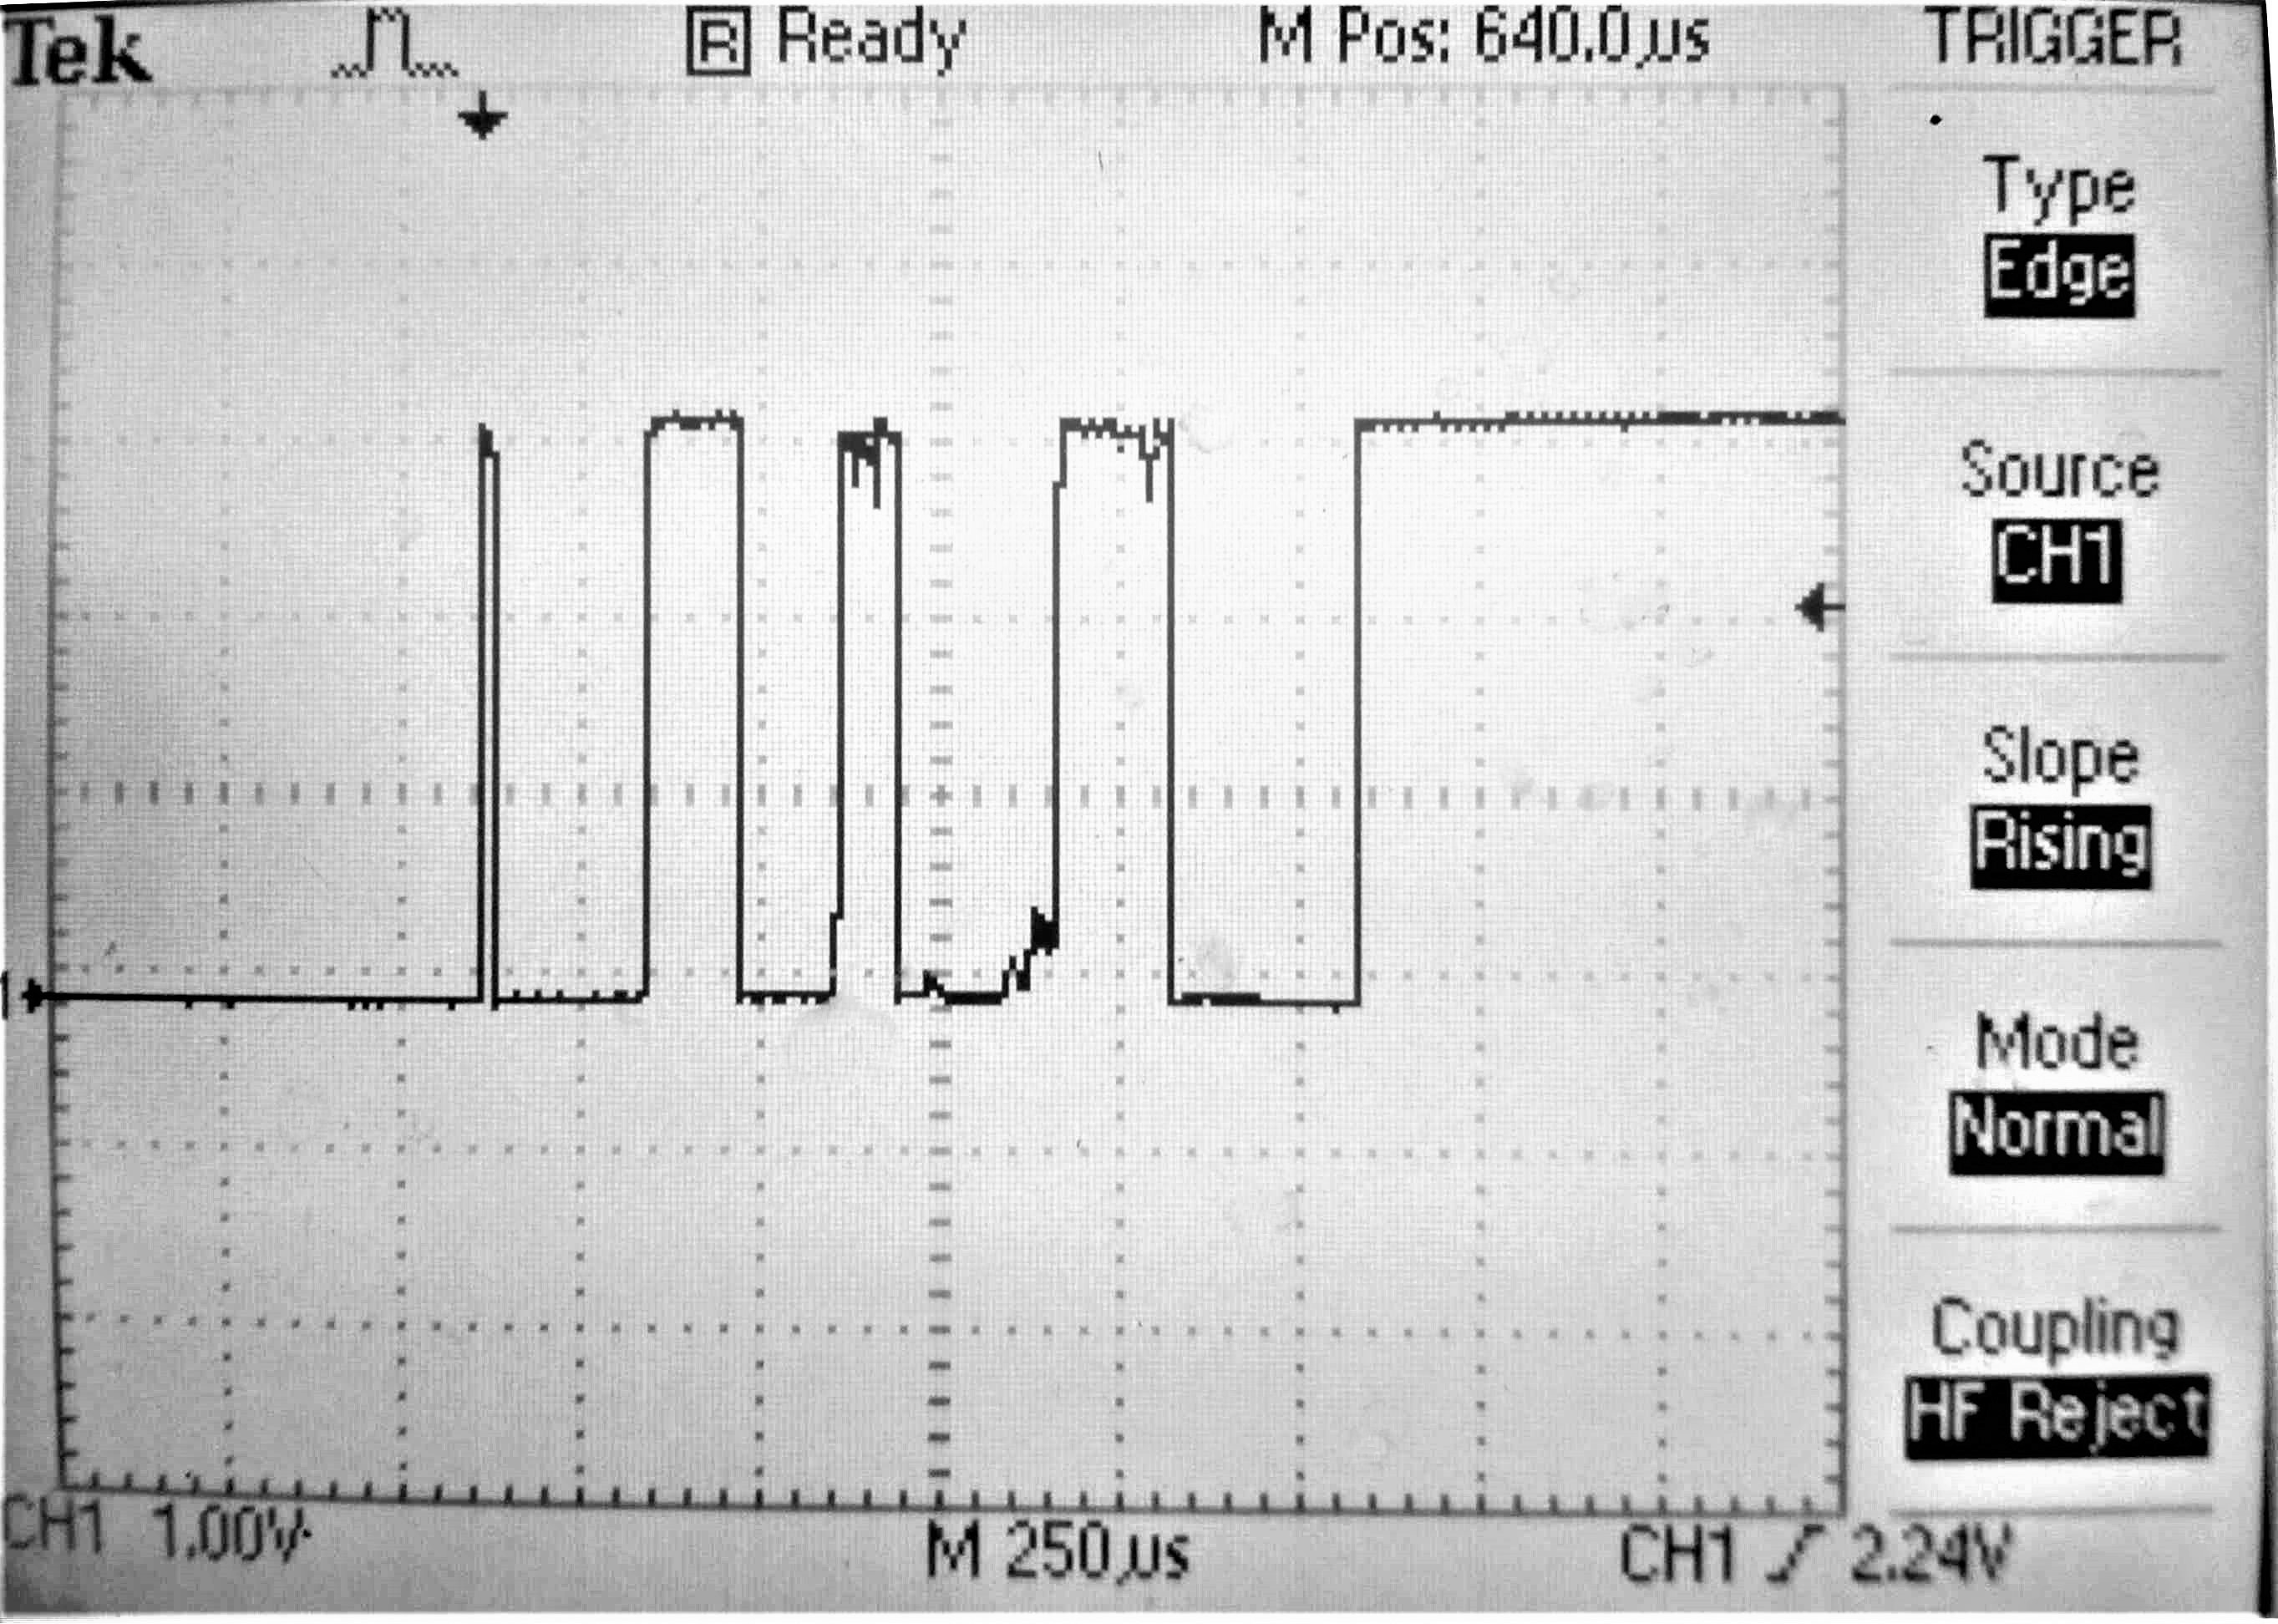
\includegraphics[width=0.45\textwidth]{rys03/drganiaPrzyciskow.jpg} & 
				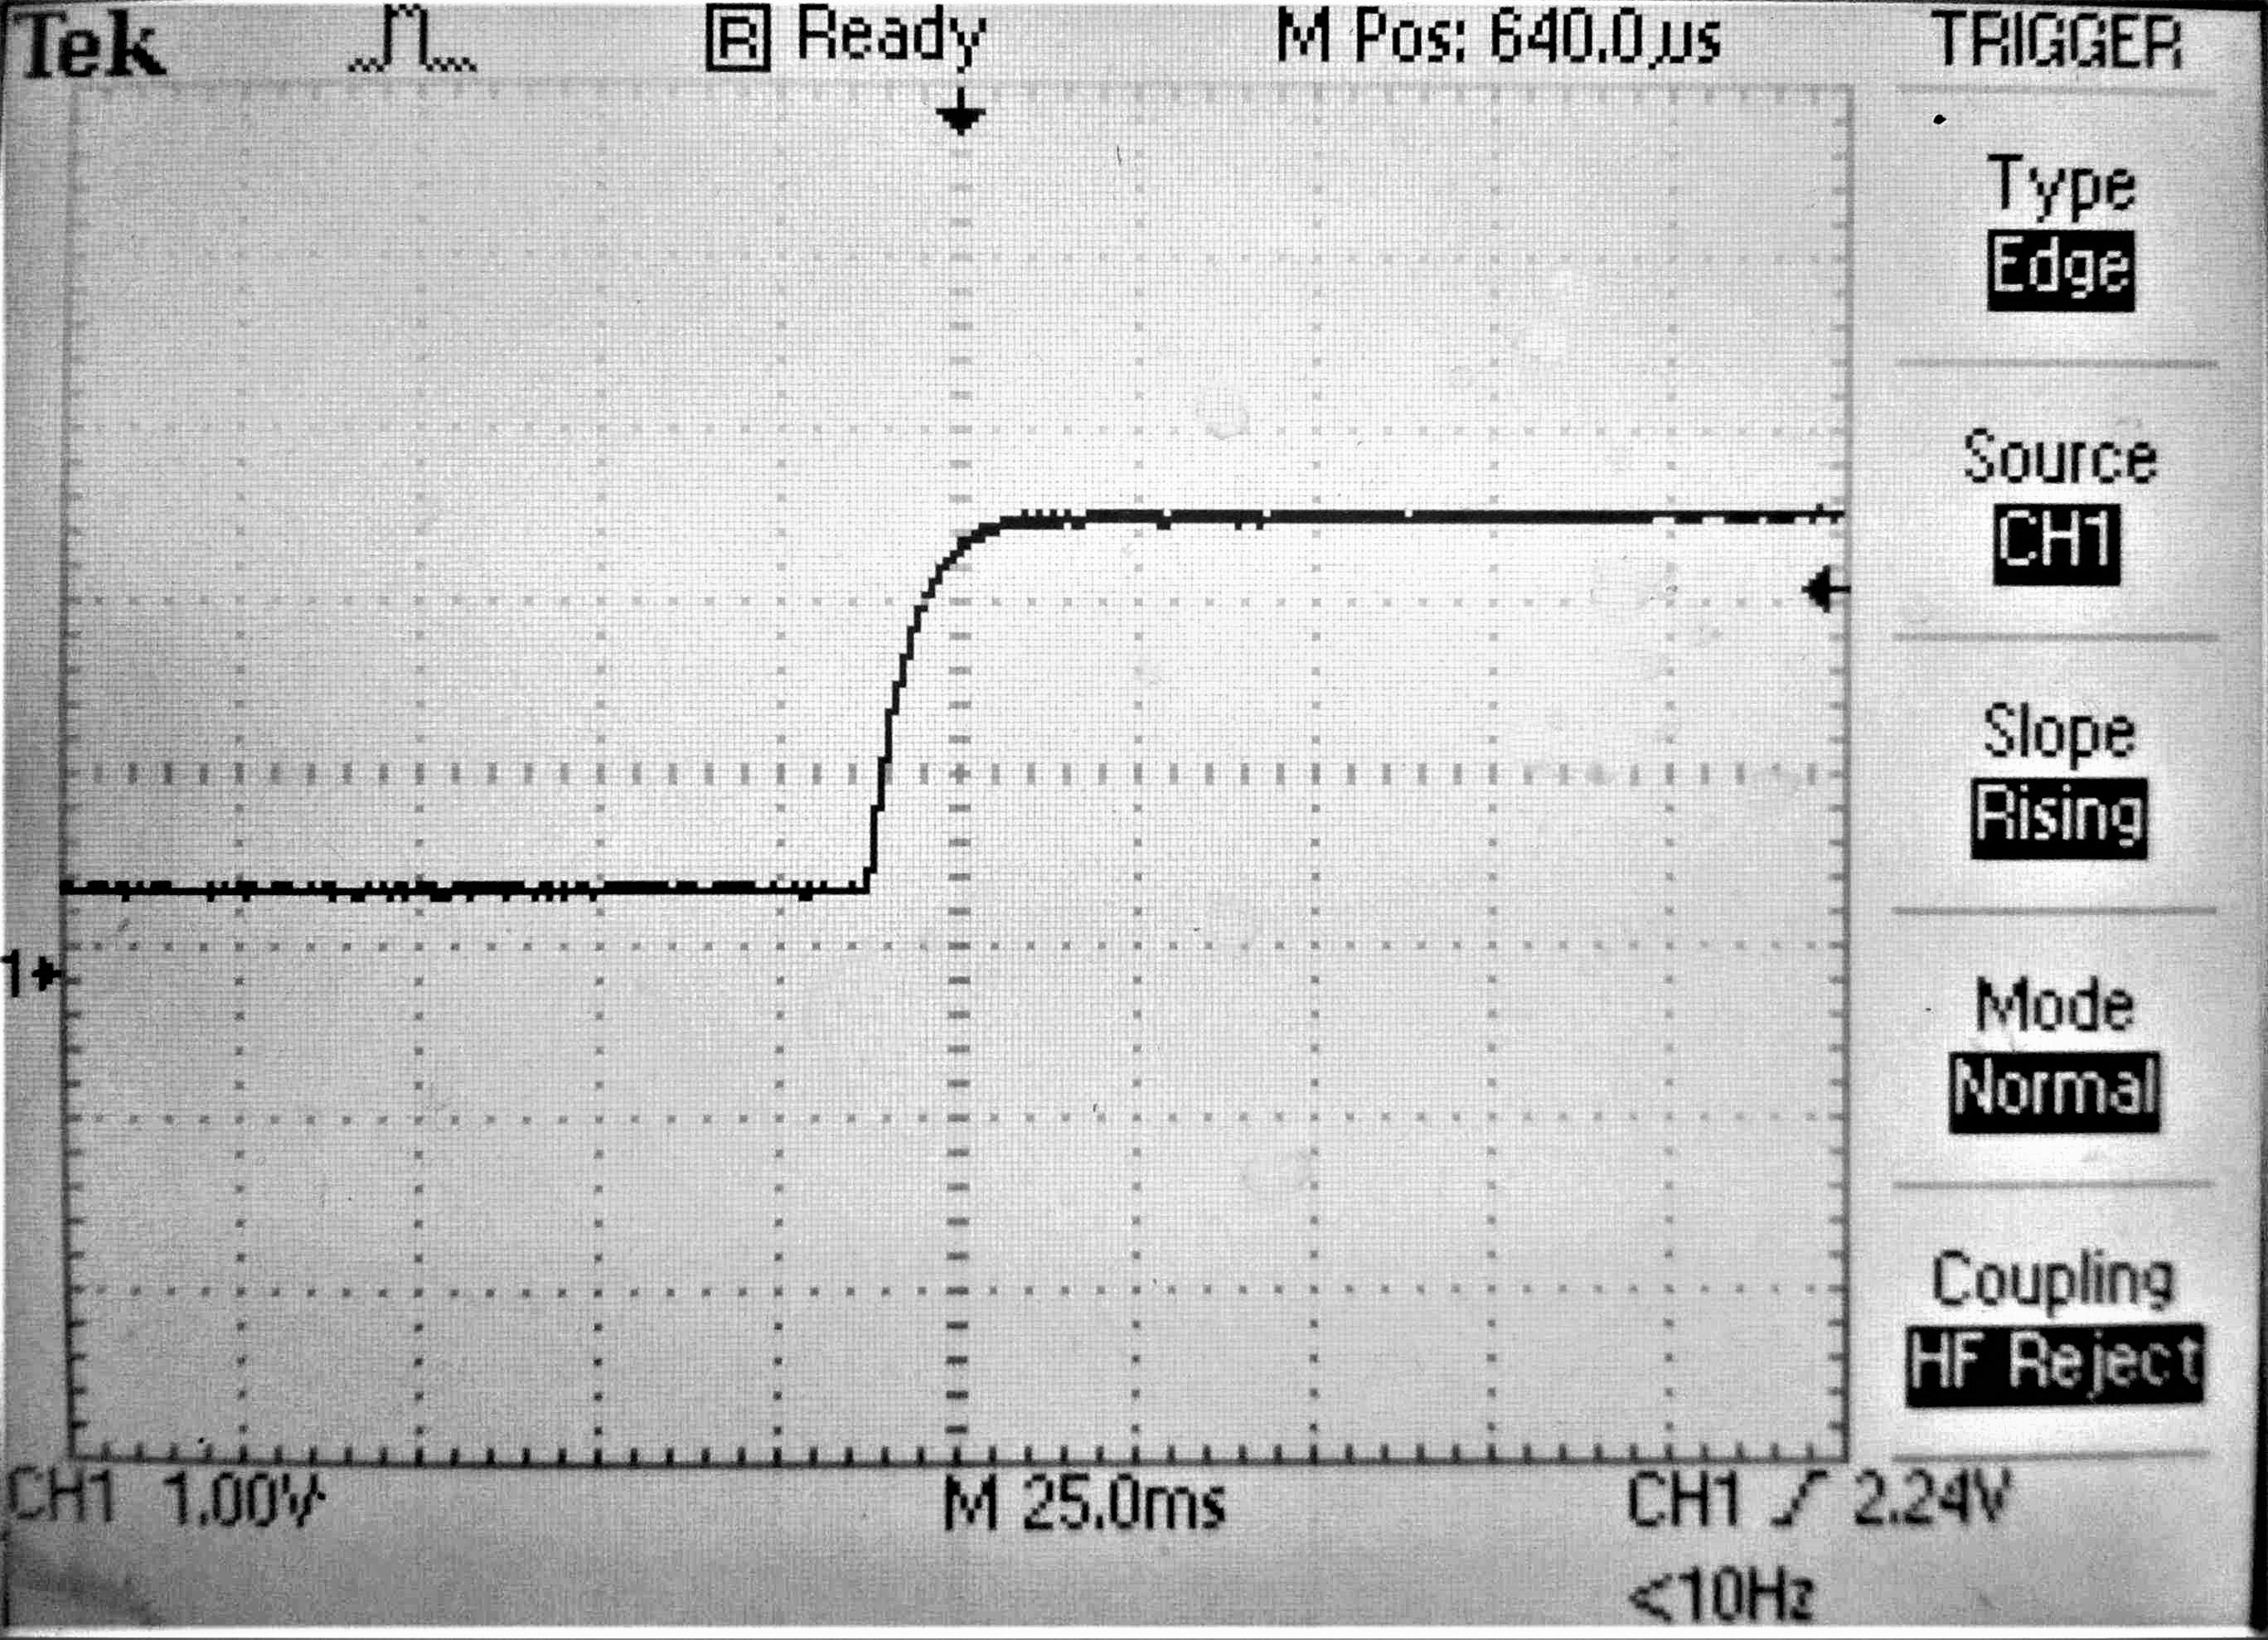
\includegraphics[width=0.45\textwidth]{rys03/drganiaStykowFiltr.jpg} \\
			\end{tabular}
			\caption{Drania styków a) przed filtracją b) po filtracji}
			\label{fig:drganiaStykow}
		\end{figure}
		
	\section{Filtracja zasilania}
    	Przetwornice DC-DC na wyjściu posiadają pewne nierówności zasilania. Dlatego warto zastosować filtrację w postaci dławików i kondensatorów. Badania przeprowadzono dla przetwornicy obniżającej napięcie MP2307. Do filtracji użyto dławika \textcolor{red}{wartość} oraz kondensatora \SI{2200}{\micro\farad}.
	    \begin{figure}[ht]
			\centering
			\begin{tabular}{@{}ll@{}}
				a) & b) \\
				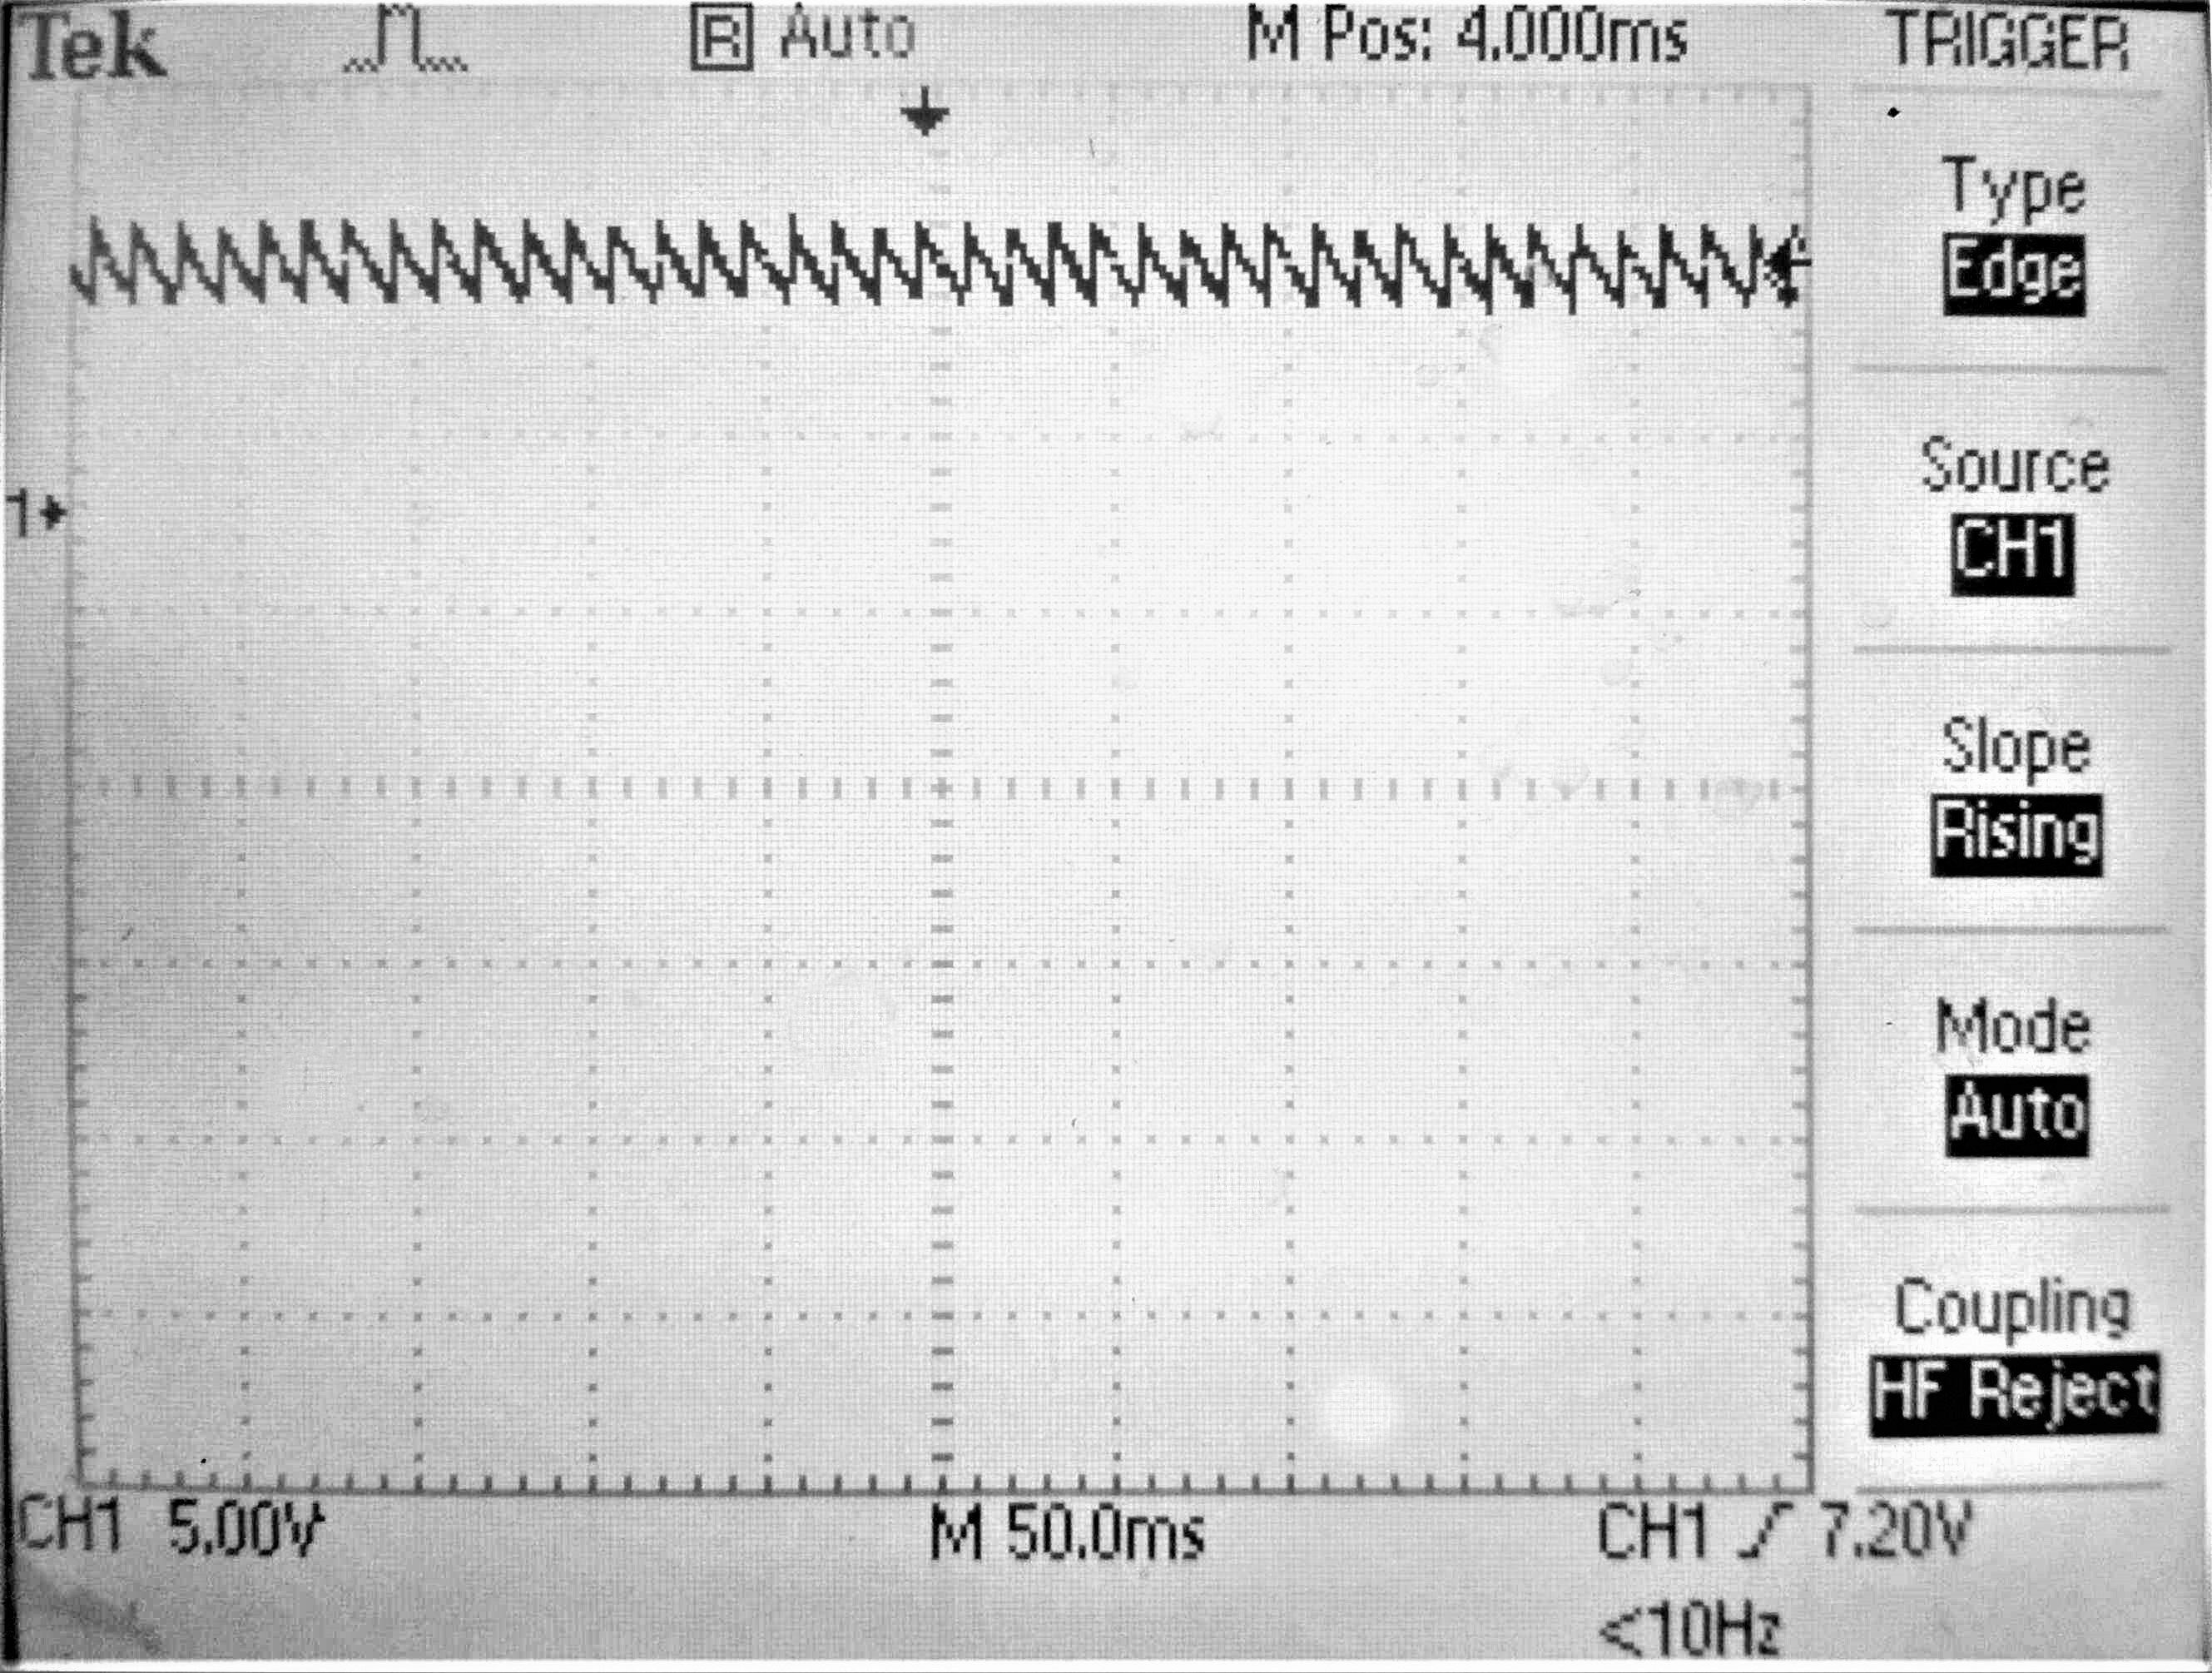
\includegraphics[width=0.45\textwidth]{rys03/zasilanie.jpg} & 
				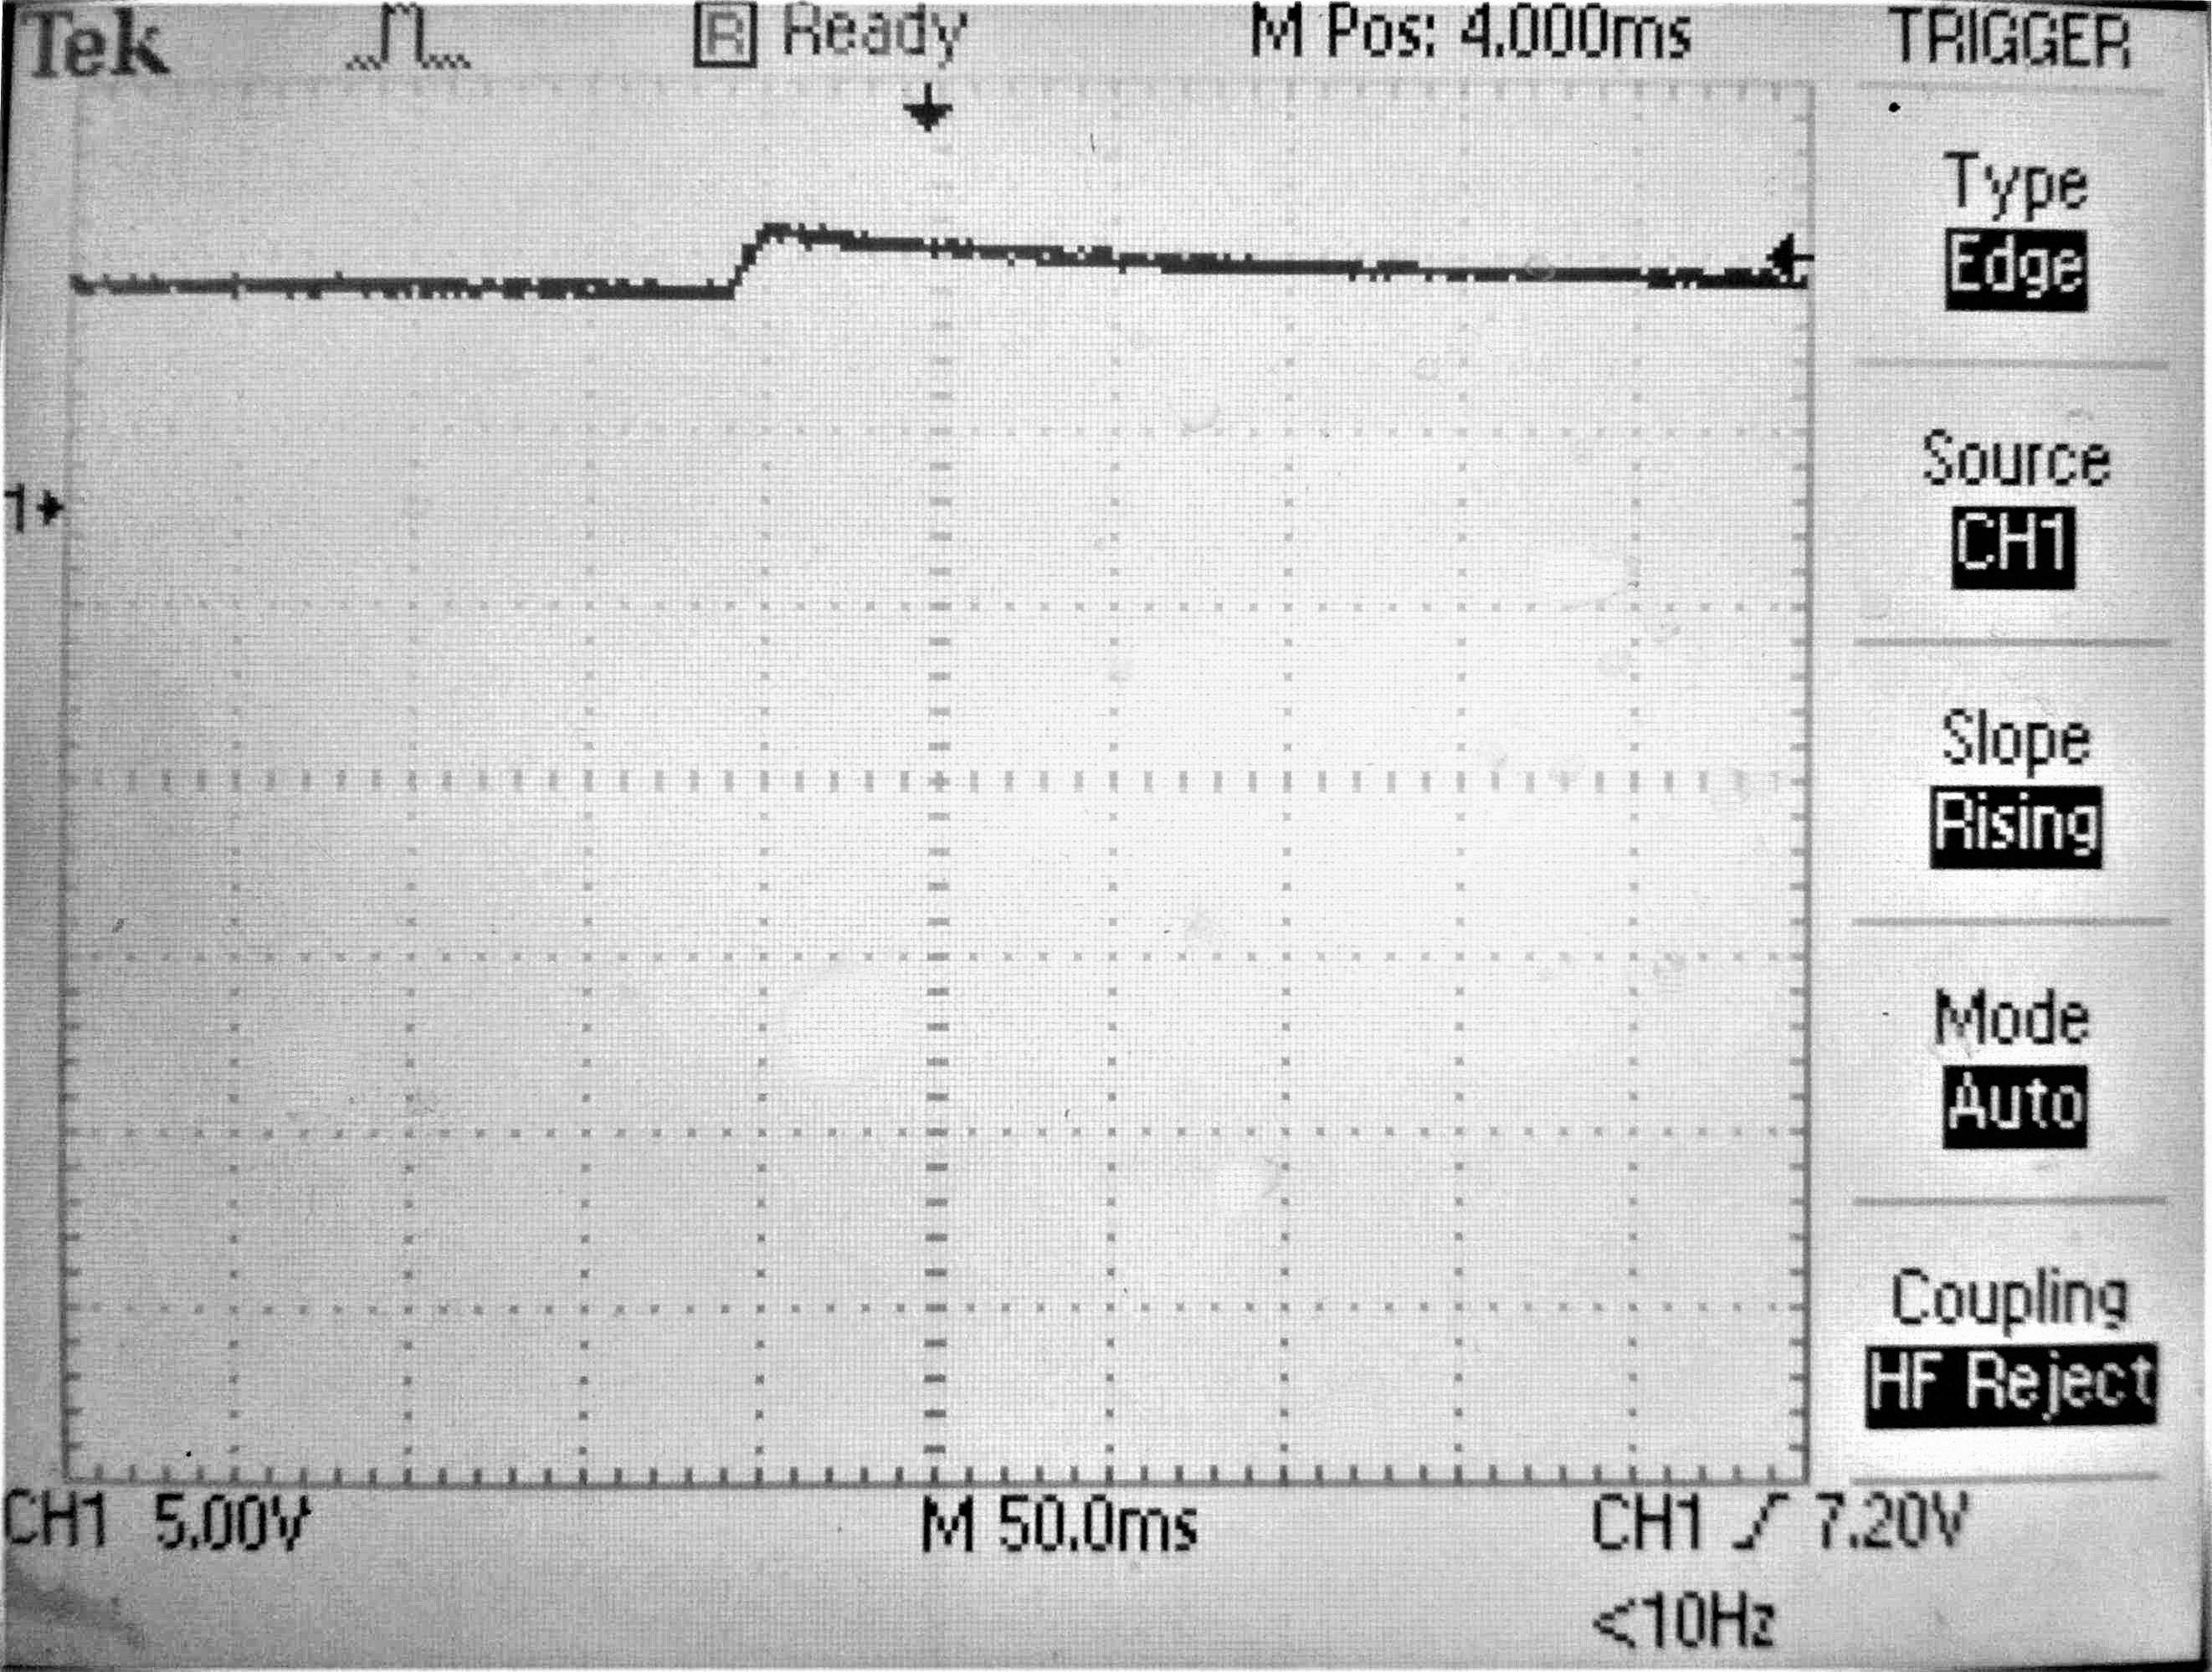
\includegraphics[width=0.45\textwidth]{rys03/zasilanieFiltr.jpg} \\
			\end{tabular}
			\caption{Napięcie zasilania a) przed filtracją b) po filtracji}
			\label{fig:filtracjaZasilania}
		\end{figure}
		Jak widać na rysunku \ref{fig:filtracjaZasilania} filtr znacznie ograniczył częstotliwość wahań napięcia. Jednak nie udało się ich wyeliminować całkowicie i pojawiają się okresowo. 
		
	\section{Zabezpieczenia tranzystorów}
	    W przypadku wykorzystywania elementów indukcyjnych m.in silników, należy zwrócić uwagę na ich zachowanie w przypadku zmian prądów w obwodzie. Następuje wtedy zjawisko samoindukcji i w cewce jest generowana siła elektromotoryczna. Zależność indukowanej siły elektromotorycznej od zmiany prądu przedstawia wzór \ref{eq:SEMcewki}.
	    \begin{equation}
	        E = -L \frac{di}{dt}
	        \label{eq:SEMcewki}
	    \end{equation}
	    gdzie: \\
	    E  – siła elektromotoryczna, \\
	    L – indukcyjność cewki, \\
        i – natężenie prądu płynącego przez cewkę, \\
        t – czas. \\
        Wynika z niego, że gwałtowne zmiany prądu występujące np. podczas sterowania sygnałem PWM powodują generowanie wysokich impulsów napięcia na cewce. Badania przeprowadzone na pompce wody potwierdzają rozważania teoretyczne. Przebieg napięcia podczas sterowania sygnałem PWM o wypełnieniu \SI{50}{\percent} został przedstawiony na rysunku \ref{fig:pompkaBezFiltracji}.
        \begin{figure}[ht]
			\centering
			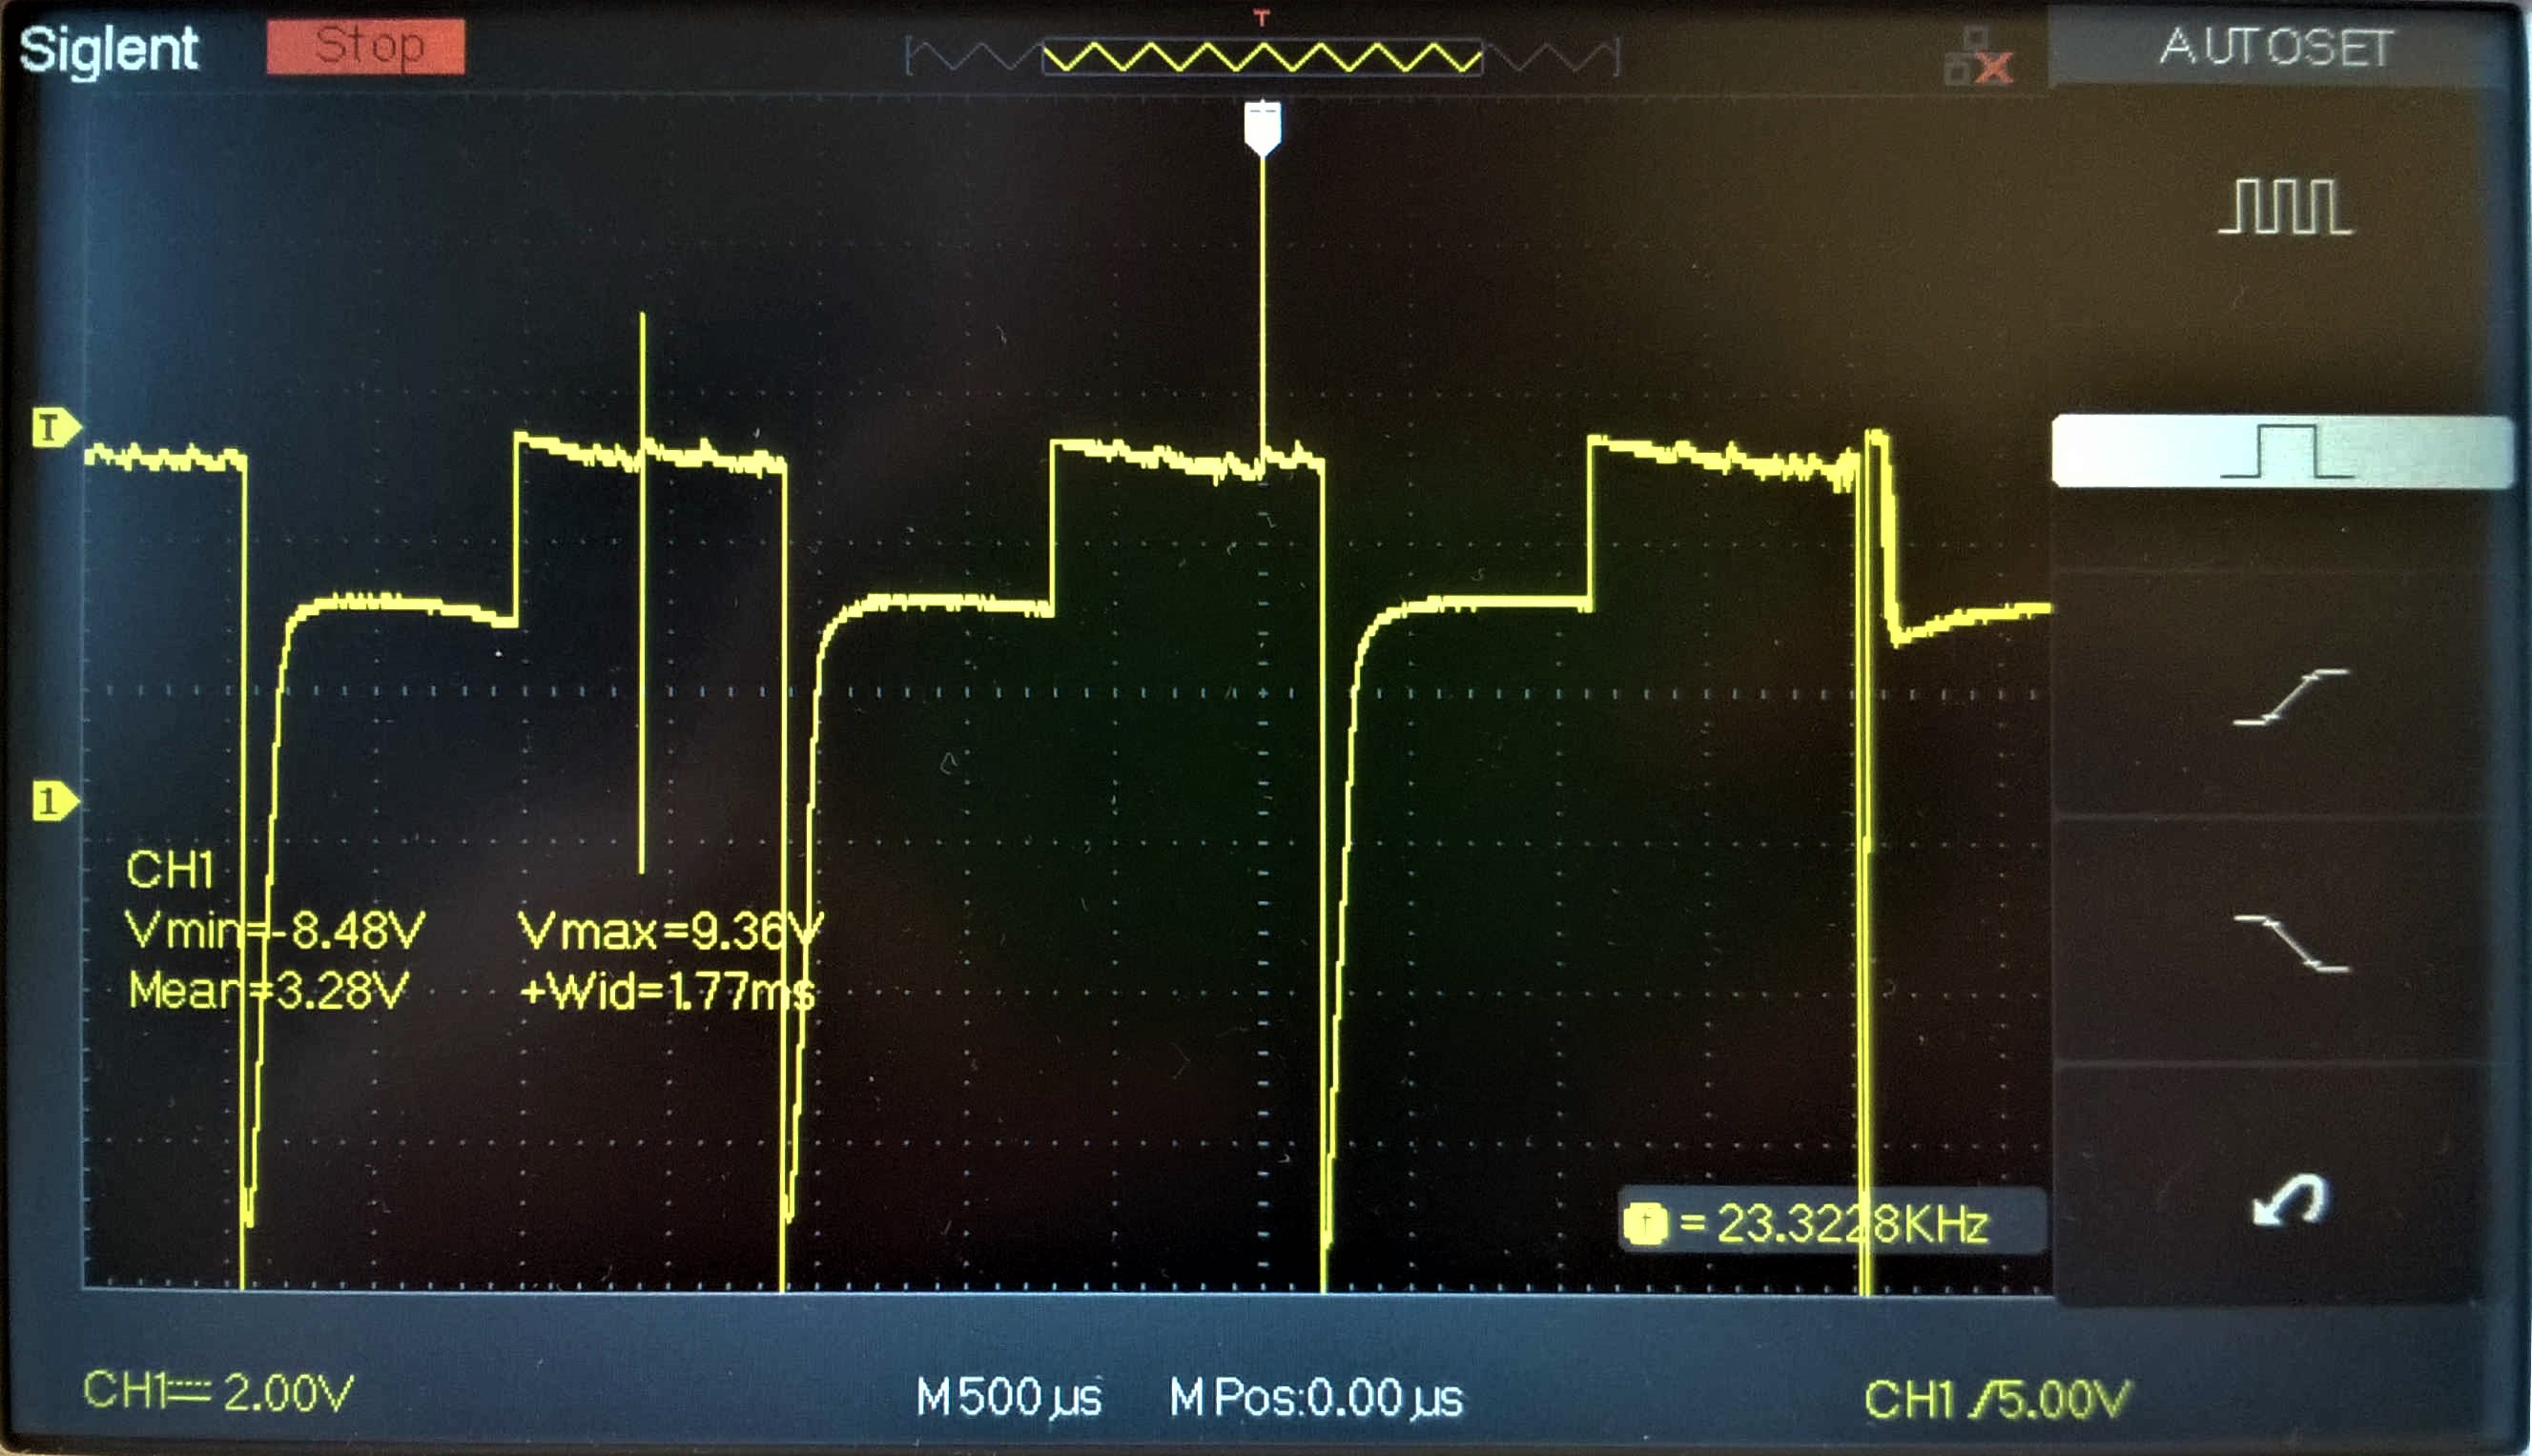
\includegraphics[width=0.45\textwidth]{rys03/przedSchottky.jpg}
			\caption{Napięcie na pompce wody bez filtracji}
			\label{fig:pompkaBezFiltracji}
		\end{figure}
		Widać na nim gwałtowne impulsy napięcia, znacznie przewyższające wartości sygnału PWM. Takie zachowanie może zniszczyć tranzystor sterujący. Dlatego aby zniwelować ten efekt stosuje się połączoną równolegle do zacisków elementu indukcyjnego diodę Schottkyego, dodatkowo można podłączyć także kondensator. Wyniki dla takich zabezpieczeń zostały przedstawione na rysunku \ref{fig:pompkaFiltracja}.
		\begin{figure}[ht]
			\centering
			\begin{tabular}{@{}ll@{}}
				a) & b) \\
				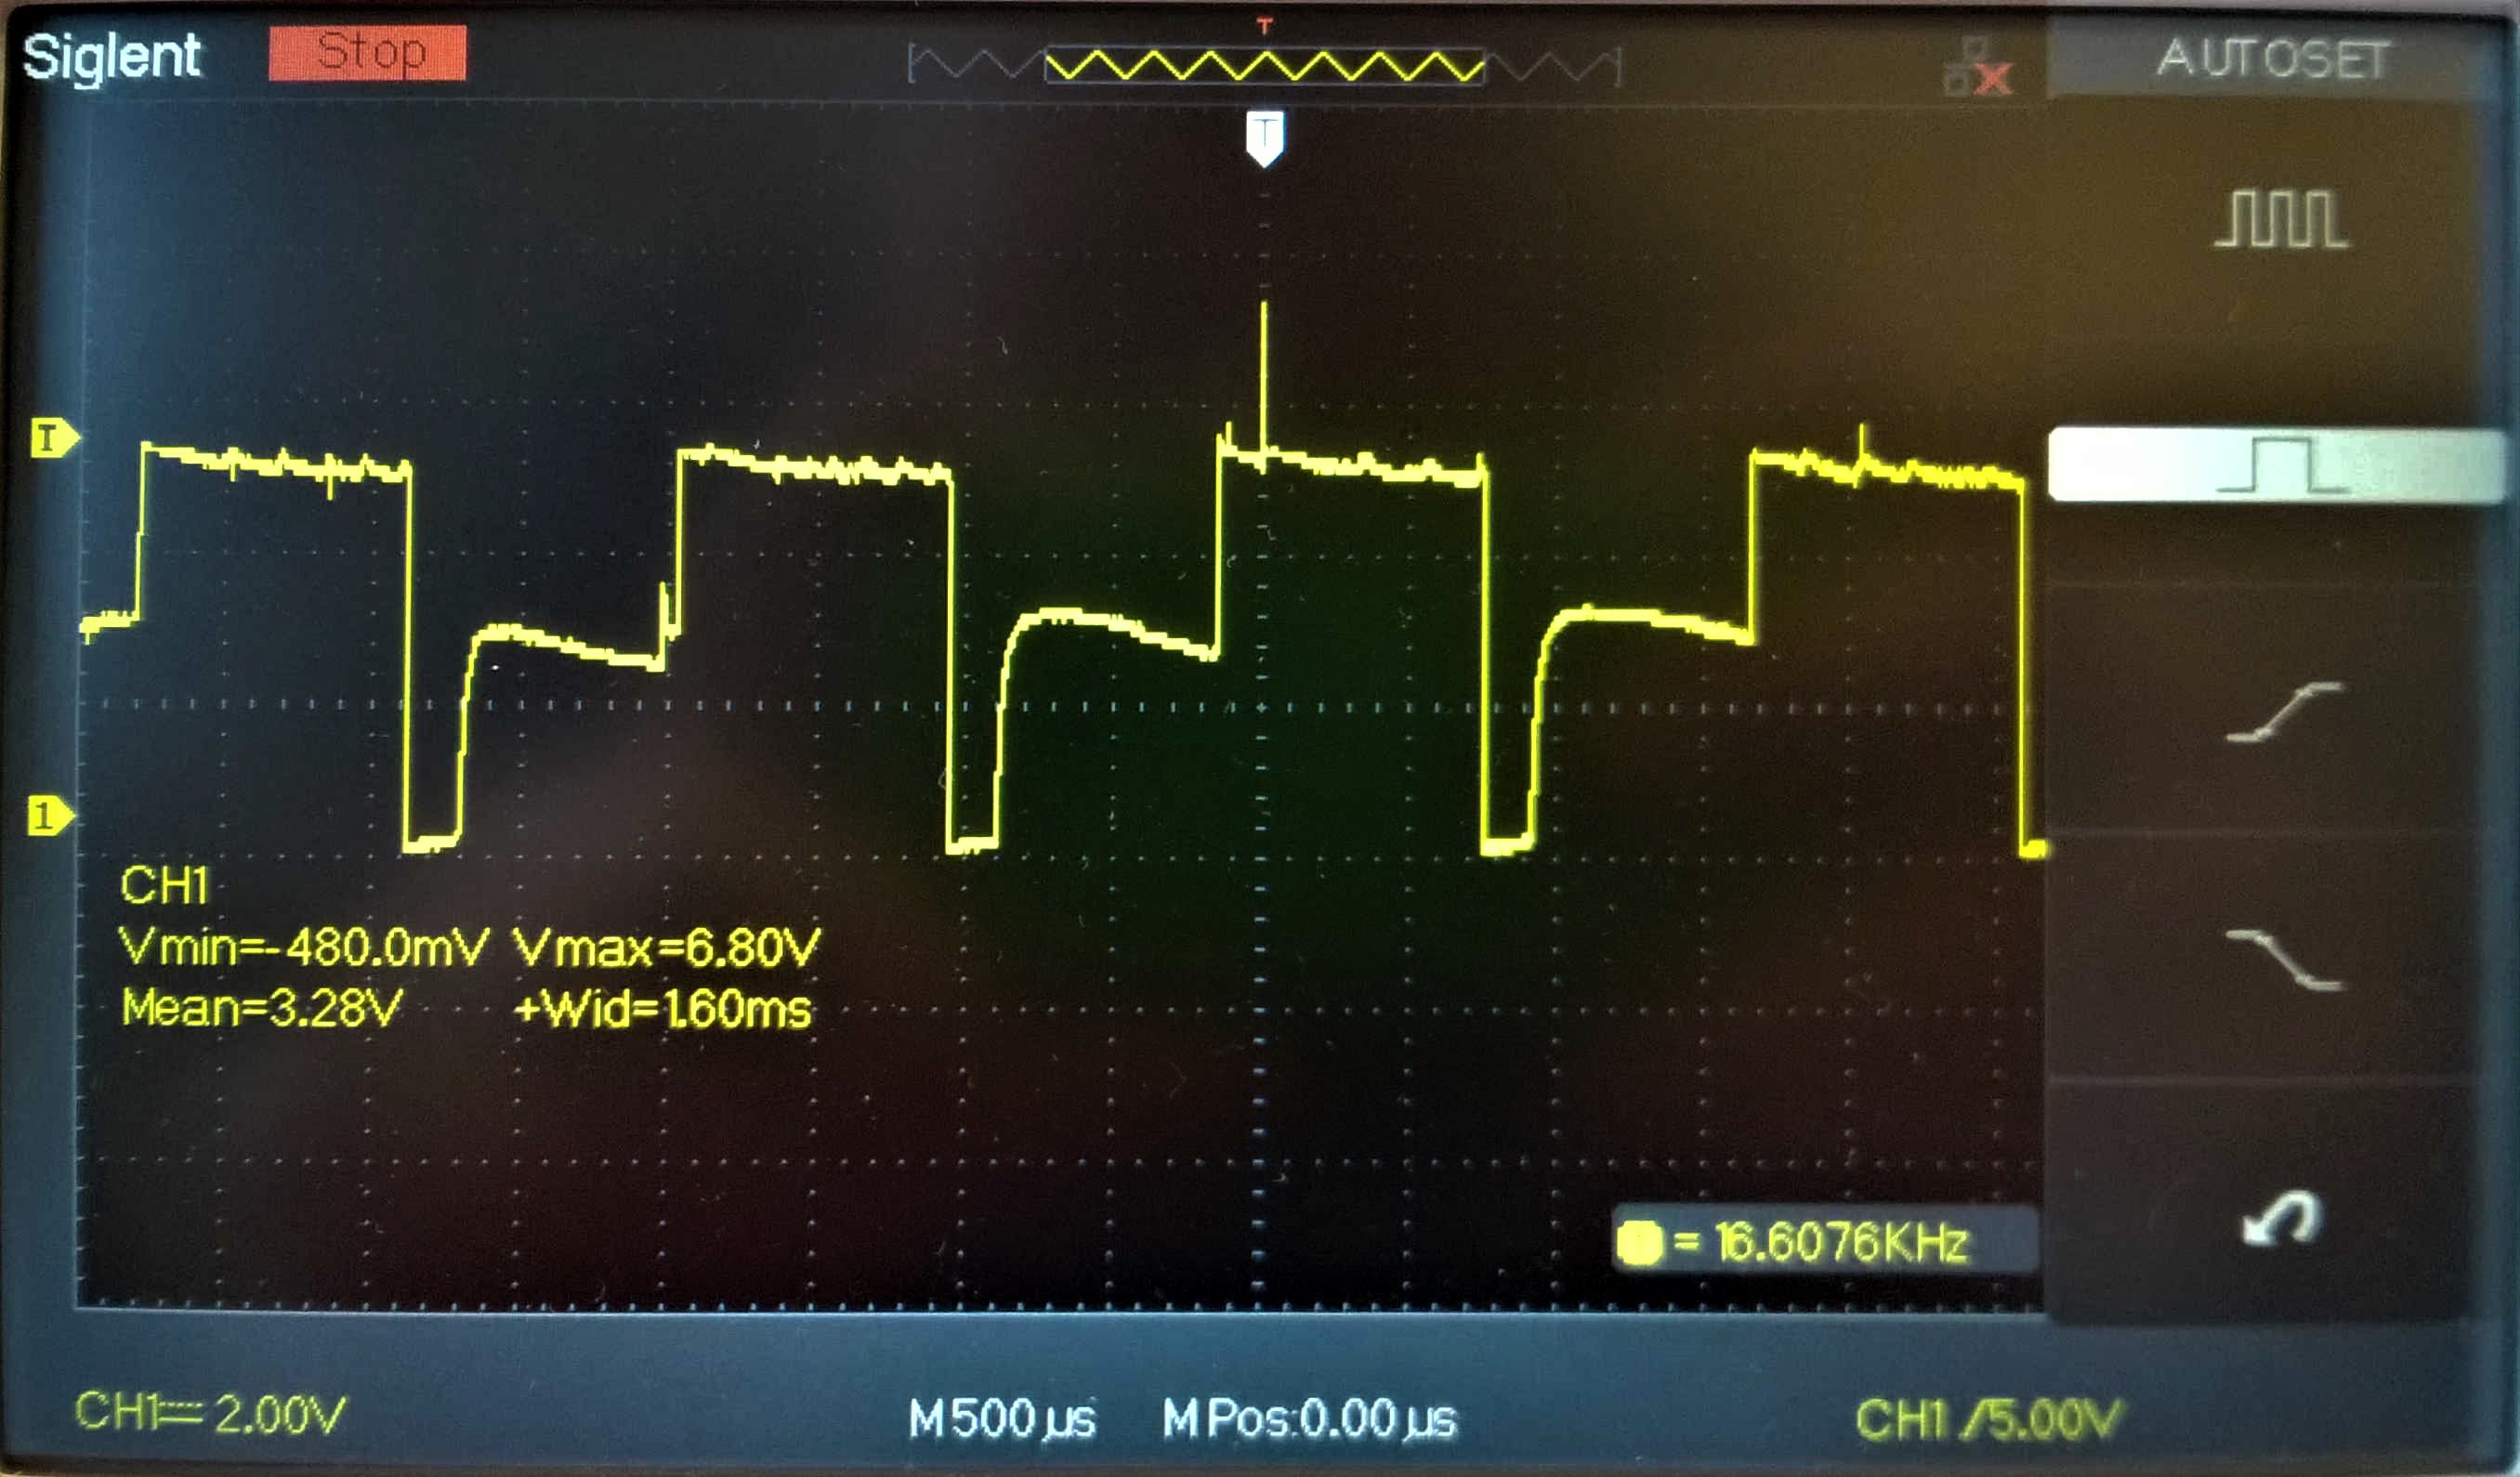
\includegraphics[width=0.45\textwidth]{rys03/schottky.jpg} & 
				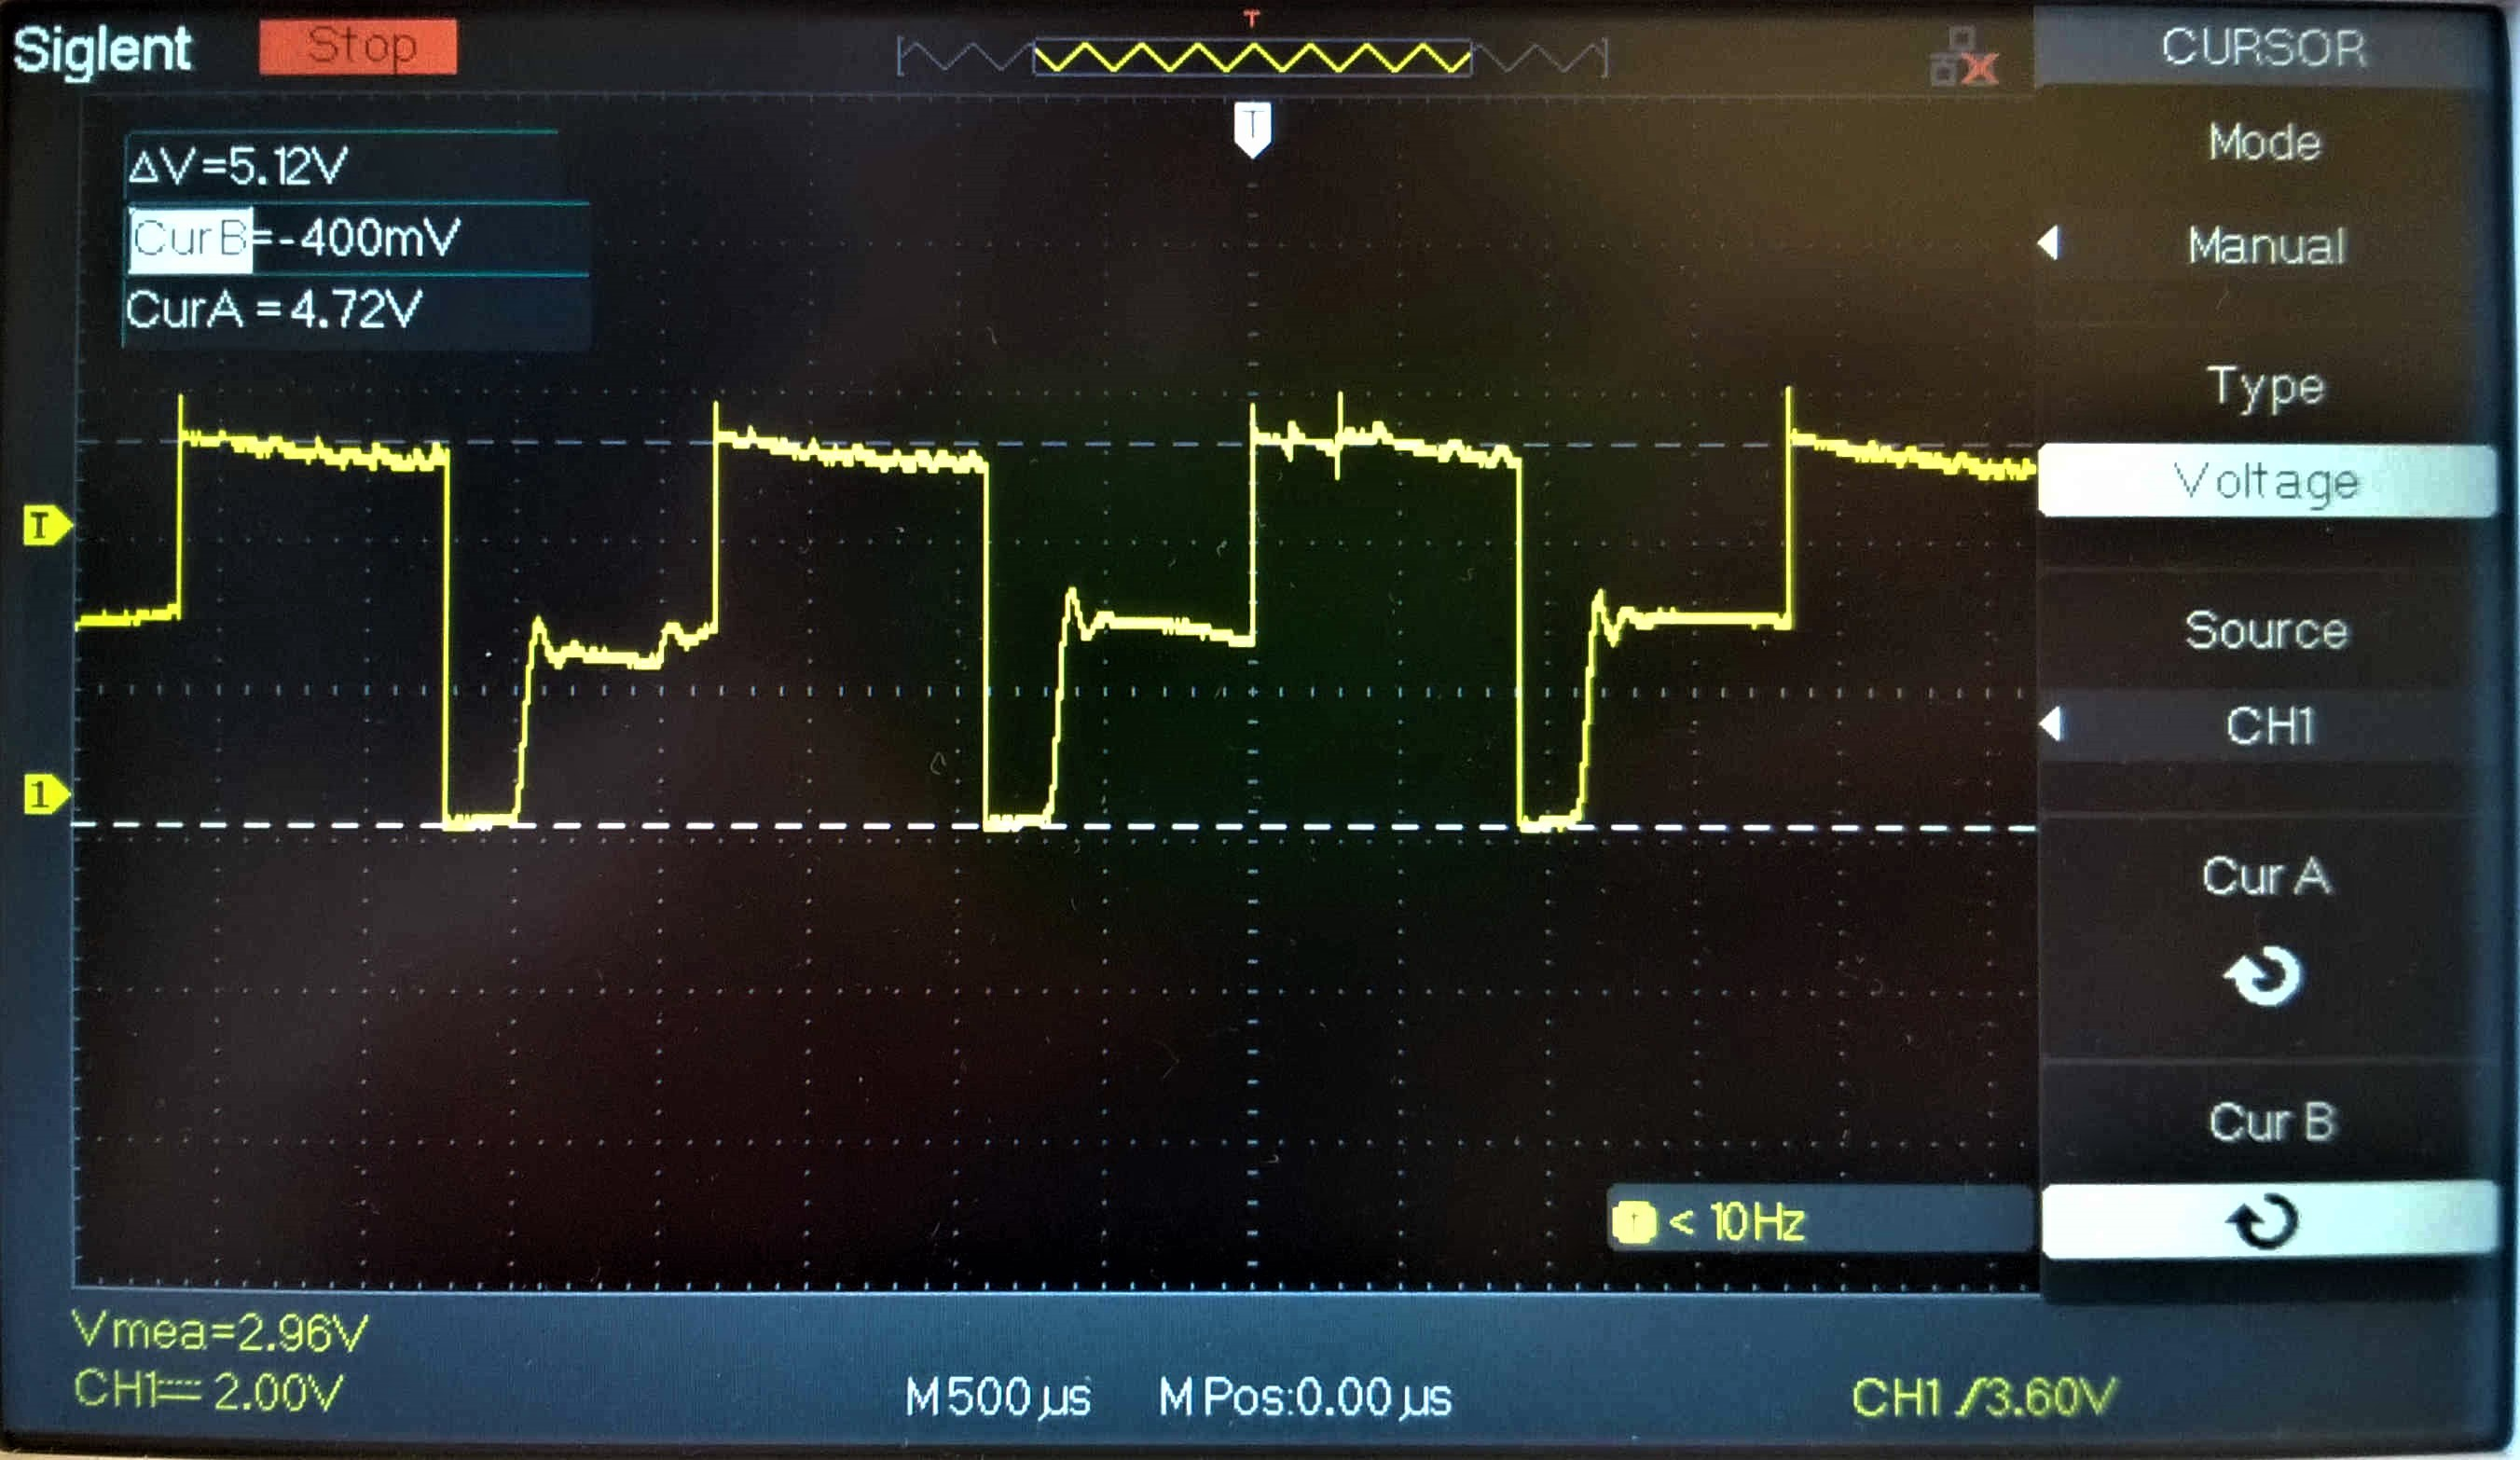
\includegraphics[width=0.45\textwidth]{rys03/schottkyZkondem.jpg} \\
			\end{tabular}
			\caption{Napięcie na pompce wody: a) z diodą Schottkyego b) z diodą Schottkyego i kondensatorem}
			\label{fig:pompkaFiltracja}
		\end{figure}
		Widać na nich ograniczenie przepięcia do wartości napięcia przewodzenia diody.
		
		W projekcie zastosowane zostały gotowe moduły sterowania silnikami, które rozwiązują przedstawiony problem.